\chapter{Opgave-oplæg}

\vspace{-20pt}

På Ingeniørhøjskolen Aarhus Universitet er en AeroQuad Cyclone ARF quadrocopter tilgængelig.
Førhen er quadrocopteren blevet fjernstyret via line of sight, radiokommunikation. Målet med projektet er, at lave quadrocopteren til en autonom overvågnings drone.

Groft skitseret består projektet af følgende to dele: 
1. Quadrocopter
2. Webapplikation

Fra start består quadrocopteren af et stel, nogle motorer og et batteri. GPS, kamera og 3G modul tilføjes quadrocopteren for at udvide dens funktionalitet. GPS tilføjes, så dronen hele tiden kan tilpasse flyveorientering ud fra sammenligning af nuværende og ønsket position. Kameraet skal bruges til at dokumentere at dronen har været ved waypoints. Det skal være muligt enten at tage billeder eller optage film sekvenser. Det ønskes, at drone og webapplikation skal kommunikere via internettet. For at forbinde drone til internettet tilkobles et 3G modul.

Webapplikation har to formål. For det første, skal webapplikation bruges til at indstille nye flyveruter. Nye flyveruter dannes ud fra waypoints som vælges af bruger. Ved indstilling af nye flyveruter skal flyvehøjde, billedkvalitet mm. også indstilles. For det andet skal webapplikationen bruges til at tilgå en database, hvor billeder, film og flyveruter gemmes.

Nederst til højre på systemskitsen ses et device. Dette device har internet adgang og bruges til at tilgå webapplikation hvor opsætning af ny flyvning ordnes.  Når en bruger har lavet indstillinger til ny flyvning, overføres opsætningen via internettet til quadrocopteren. Quadrocopteren finder via GPS ud af hvor den er, og hvor den skal flyve hen. Under flyvningen tager quadrocopteren billeder eller optager video, som via nettet overføres til webapplikationens database.

\vspace{-5pt}
%Systemskitse
\begin{figure}[H]
\centering
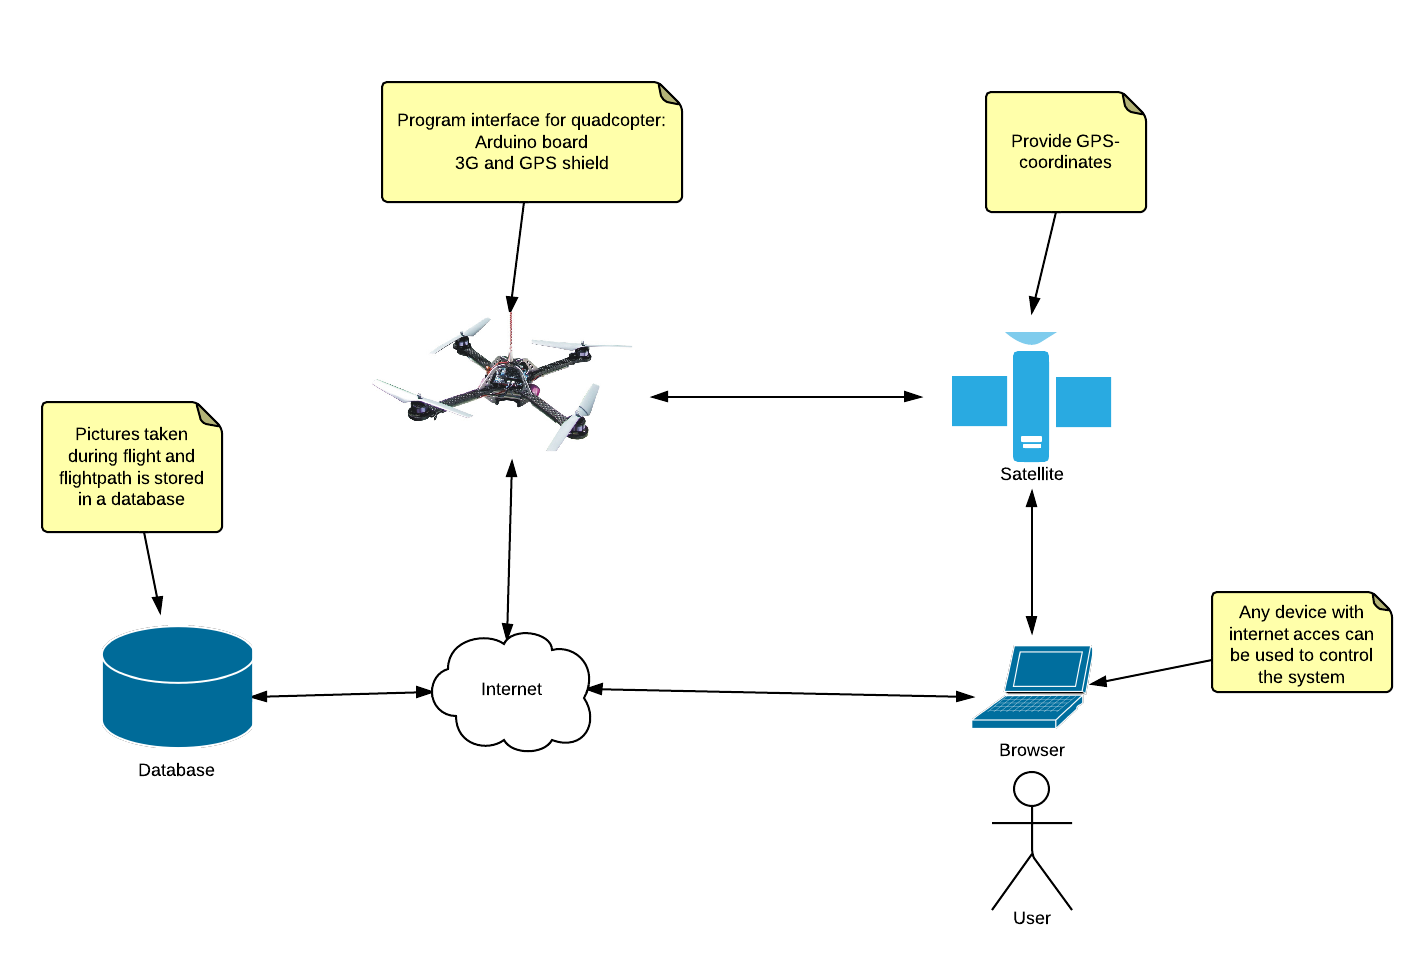
\includegraphics[width=0.75\textwidth]{Billeder/Projektbeskrivelse.png}
\vspace{-5pt}
\caption{Systemskitse}
\label{fig:Systemskitse}
\end{figure}